\chapter{Alternating Current and Time Varying Signals}

\section{Introduction}

In this lab you will use two essential new pieces of lab equipment:
the digital oscilloscope and the function generator.  You will learn
how to measure AC voltages with your DMM, how to view
time-dependent wave forms on your digital oscilloscope and how to trigger digital oscilloscope. For this lab there are both logbook and jupyter notebook entries.


\section{Function Generator}

\begin{figure}[htbp]
\begin{center}
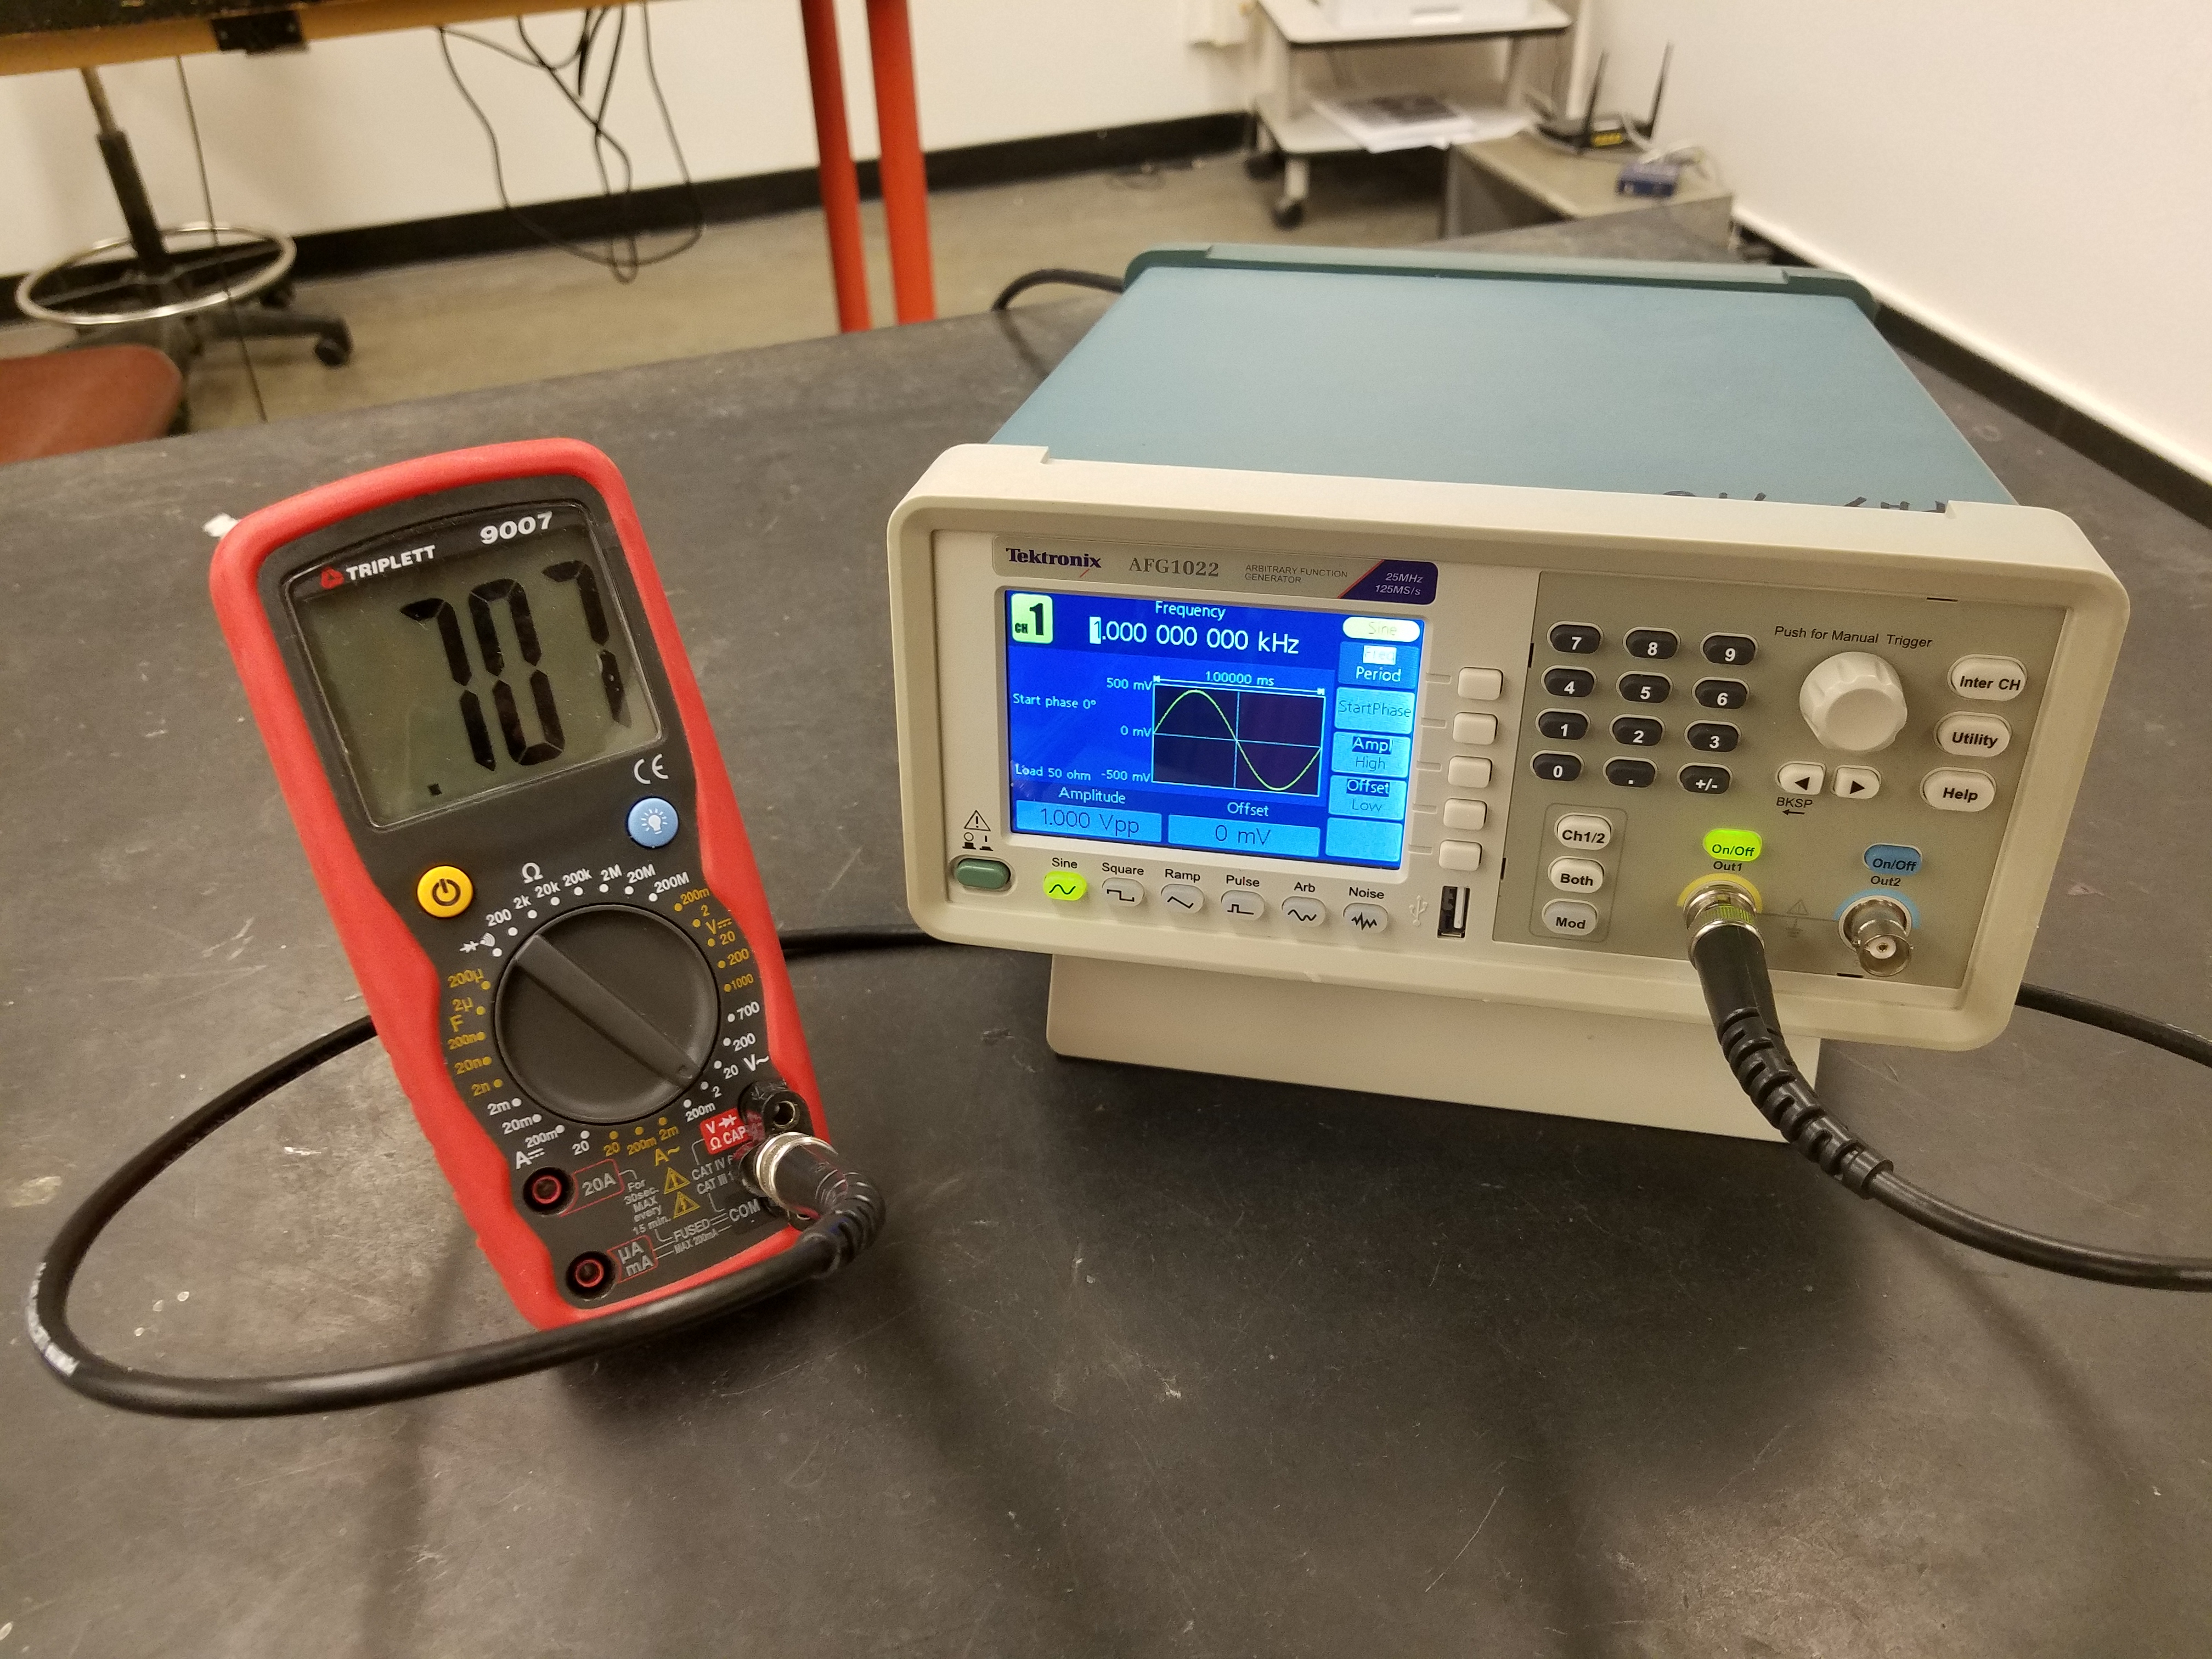
\includegraphics[width=0.45\textwidth]{figs/labs/lissajous/generator_dmm_setup.jpg} 
\caption{Connect the Channel 1 Output of your function generator directly to your DMM.}
\label{fig:dmm_setup}
\end{center}
\end{figure}

 Connect the output of Channel 1 directly to the Voltage measurement
input of your Triplett 9007 DMM, using a coaxial cable with BNC connectors, and a BNC to banana plug adapter as
shown in Fig.~\ref{fig:dmm_setup}.  BNC is a type of quick connector often used for coaxial cable.  Coaxial cable is a type of electrical cable that can transmit high frequency signals with low losses. It has an inner conductor surrounded by a insulating layer, surrounded by a conducting shield. Every coaxial cable has a characteristic impedance and the one you will use in the lab has $50~\rm \Omega$. 

Turn on power to the function
generator.  Then set your function generator to the factory default:
\begin{displaymath}
\rm Utility\;Button \to System \to Set\;to\;Default \to Select.
\end{displaymath}
You must perform this step today for the instructions that follow to
make sense.  With shared equipment, it is essential to know how to
restore the factory default, in case another user has left the device
with strange settings.  You don't need to start with this step every
lab, but it is a fast way to recover when you encounter strange
behavior in your equipment.

The factory default settings are set to produce a Sine function with a
peak-to-peak voltage $v_{\rm pp} = 1.0~\rm V$ and a frequency $f=1~\rm
kHz$.  We'll leave that as is for now.  To turn on the output, push
the ``On/Off'' directly above the coaxial output for Channel 1, and
then ensure that the button is lit.

\begin{figure}[htbp]
\begin{center}
\begin{tabular}{ccc}
\begin{circuitikz}[line width=1pt]
\draw (0,0) coordinate(X) to[sinusoidal voltage source,bipoles/length=1.5cm] ++(0,2.0) 
to[R,l=$R_{\rm S}$] ++(0,2.0) to[short,-o] ++(1.0, 0) node[right]{B};
\draw (0.2,3.0) node[right] {$50~\rm \Omega$};
\draw (X) node[ground,yscale=2.0]{} to[short,-o] ++(1.0,0) node[right]{A};
\draw (0,-0.5) node[]{};
\end{circuitikz} &
\begin{circuitikz}[line width=1pt]
\draw (0,0) coordinate(X) to[short] ++(0,2.0) node[component]{V} to[short] ++(0,2.0) to[short,-o] ++(-1.0, 0) node[left]{B};
\draw (X) to[short,-o] ++(-1.0,0) node[left]{A};
\draw (0,-0.5) node[]{};
\end{circuitikz} &
\begin{circuitikz}[line width=1pt]
\draw (0,0) coordinate(X) to[short] ++(0,2.0) node[component]{V} to[short] ++(0,2.0) to[short] ++(-1.0, 0);
\draw (X) to[short,-*] ++(-1.0,0) coordinate(X) to[R,l=$R_L$] ++(0,4.0) to[short,*-o] ++(-1.0,0) node[left]{B};
\draw (X) to[short,-o] ++(-1.0,0) node[left]{A};
\draw (0,-0.5) node[]{};
\end{circuitikz} \\
(a) & (b) & (c) \\
\end{tabular}
\caption{Equivalent circuit for (a) your function generator, which includes a $50~\rm \Omega$ source resistance, and two typical terminations for a coaxial signal:  (b) infinite resistance voltmeter or scope, or (c) a terminating resistor in parallel.}
\label{fig:funccirc}
\end{center}
\end{figure}

\begin{measurement} Set your DMM to the $2~\rm V$ (AC) scale (the V with a squiggly line).
And you should now measure the AC voltage 
\begin{displaymath}
v_{\rm rms} = 0.707~\rm V \sim \frac{1}{\sqrt{2}}~\rm V
\end{displaymath} 
Record the measured value and instrumental uncertainty in your logbook together with the sketch of your circuit and short info. 
\end{measurement}
However, recalling the relationships between the peak-to-peak voltage, the peak-voltage, and the RMS voltage of an AC sine wave:
\begin{displaymath}
v_{\rm pp} = 2 \, v_{\rm p} = 2 \sqrt{2} \, v_{\rm rms}
\end{displaymath}
we expect our function generator, set to $v_{\rm pp} = 1.0$, to produce output with:
\begin{displaymath}
v_{\rm rms} = \frac{v_{\rm pp}}{2\sqrt{2}} \sim 0.353~\rm V
\end{displaymath}
Clearly someone is lying to us!  In fact, we've encountered a very
common source of factor of two mistakes.  The equivalent circuit for
your function generator is shown in Fig.~\ref{fig:funccirc}a.  Notice
that it includes a $50~\rm \Omega$ source resistance in series with
the AC voltage produced by the function generator.  This internal
resistance is important for a number of reasons, most notably making
it impossible to short-circuit the output and destroy the
equipment!

In our setup, we've connected the function generator output directly
to your DMM, which has a very high input resistance, effectively
infinite, as shown in Fig.~\ref{fig:funccirc}b.  However, the standard
termination for coaxial cables is $50~\rm \Omega$, and the default
setting for your function generator expects the load shown in
Fig.~\ref{fig:funccirc}c with $R_{\rm L} = 50~\rm \Omega$.  In
this case, the internal resistance and load resistance form a voltage
divider, so that the output voltage $V_{\rm AB}$ seen by the user is
$1/2$ the internal AC voltage. The function generator is designed to
produce an internal AC voltage which is twice the value selected by
the user, so that the output voltage is precisely the value specified
by the user.  We are seeing twice our requested value, because we have
no load resistor, and so no voltage divider, and instead see the full
value of internal AC voltage.  
\begin{measurement} To fix this discrepancy, we simply have
to configure our generator to expect a high load resistance at both
outputs:
\begin{eqnarray*}
{\rm Utility~Button \to Output Setup \to CH1Load \to HighZ} \\
{\rm CH2Load \to HighZ}
\end{eqnarray*}
Press the ``Ch1/2'' button until you return to the Channel 1 menu.  Adjust the amplitude to $1~{\rm V}$ peak-to-peak by:
\begin{displaymath}
\rm Ampl \to 1 \to Vpp
\end{displaymath}
Your DMM should now read the expected value:
\begin{displaymath}
v_{\rm rms} \sim 0.353~\rm V
\end{displaymath}
Record the measured value and instrumental uncertainty in your logbook together with a short comment. 
\end{measurement}

Press the button next to Ampl a couple of times.  There is a slightly
annoying feature of your function generator which allows you to
specify either the Amplitude and Offset or the High and Low voltage
values.  So if you want to adjust the Amplitude, you have to press the
button next to Ampl until the Ampl label is highlighted.  Often you'll
end up setting the wrong value by mistake.  But in general, whatever
parameter is highlighted along the side of the screen is the parameter
which you can specify by either the knob or the key pad.  
\begin{measurement} Keeping this
is mind, set your function generator to produce $1~\rm V$ RMS output:
\begin{displaymath}
\rm Ampl \to 1 \to Vrms.
\end{displaymath}
Now your DMM should also read a value quite close to one. Record this value and instrumental uncertainty in your logbook. 
\end{measurement}

\begin{measurement} Now let's adjust the frequency. Highlight the frequency parameter by pressing the button next to the ``Freq'' option until it is highlighted:
\begin{displaymath}
\rm Freq \to 10 \to kHz.
\end{displaymath}
You can also adjust the selected parameter with the multipurpose knob.
Turn the multipurpose knob until the frequency is around $100~\rm kHz$
and observe what happens to your DMM measurement.  Record your observation in your logbook. The reason your measurement is now inconsistent with the setting in the function generator, is that your DMM is only rated to $2~\rm kHz$.  It isn't intended for measuring
high-frequency AC signals.  Turn the frequency back down to $1~\rm kHz$. \end{measurement}

\begin{measurement} Next highlight the Offset parameter on your function generator and
adjust it to $2~\rm V$.  This will add a DC offset to your function
generator output.  After settling down, the measured value of the AC
voltage on your DMM should be unchanged at $1~\rm V$.  Switch your DMM
to measure the DC voltage and you should now measure the $2~\rm V$ DC
offset. Record the measured value in your logbook together with a comment.  Pay attention to the sign.  If you see a negative value, it
is because you installed your BNC-to-banana adapter incorrectly. 
Notice that one side of the adapter has a small raised tab, indicating
which side connects to the coaxial cable shield.  The side with the
raised tab should be plugged into the Common socket.  Whether you got
lucky this time or not, change the orientation of the adapter a few
times and observe how the sign of the voltage changes, finally
plugging it back in with the correct orientation. Now adjust the DC
level with the multipurpose knob and observe the change on your DMM.
When satisfied, set the offset back to zero. \end{measurement}

\section{Oscilloscope}

\begin{figure}[htbp]
\begin{center}
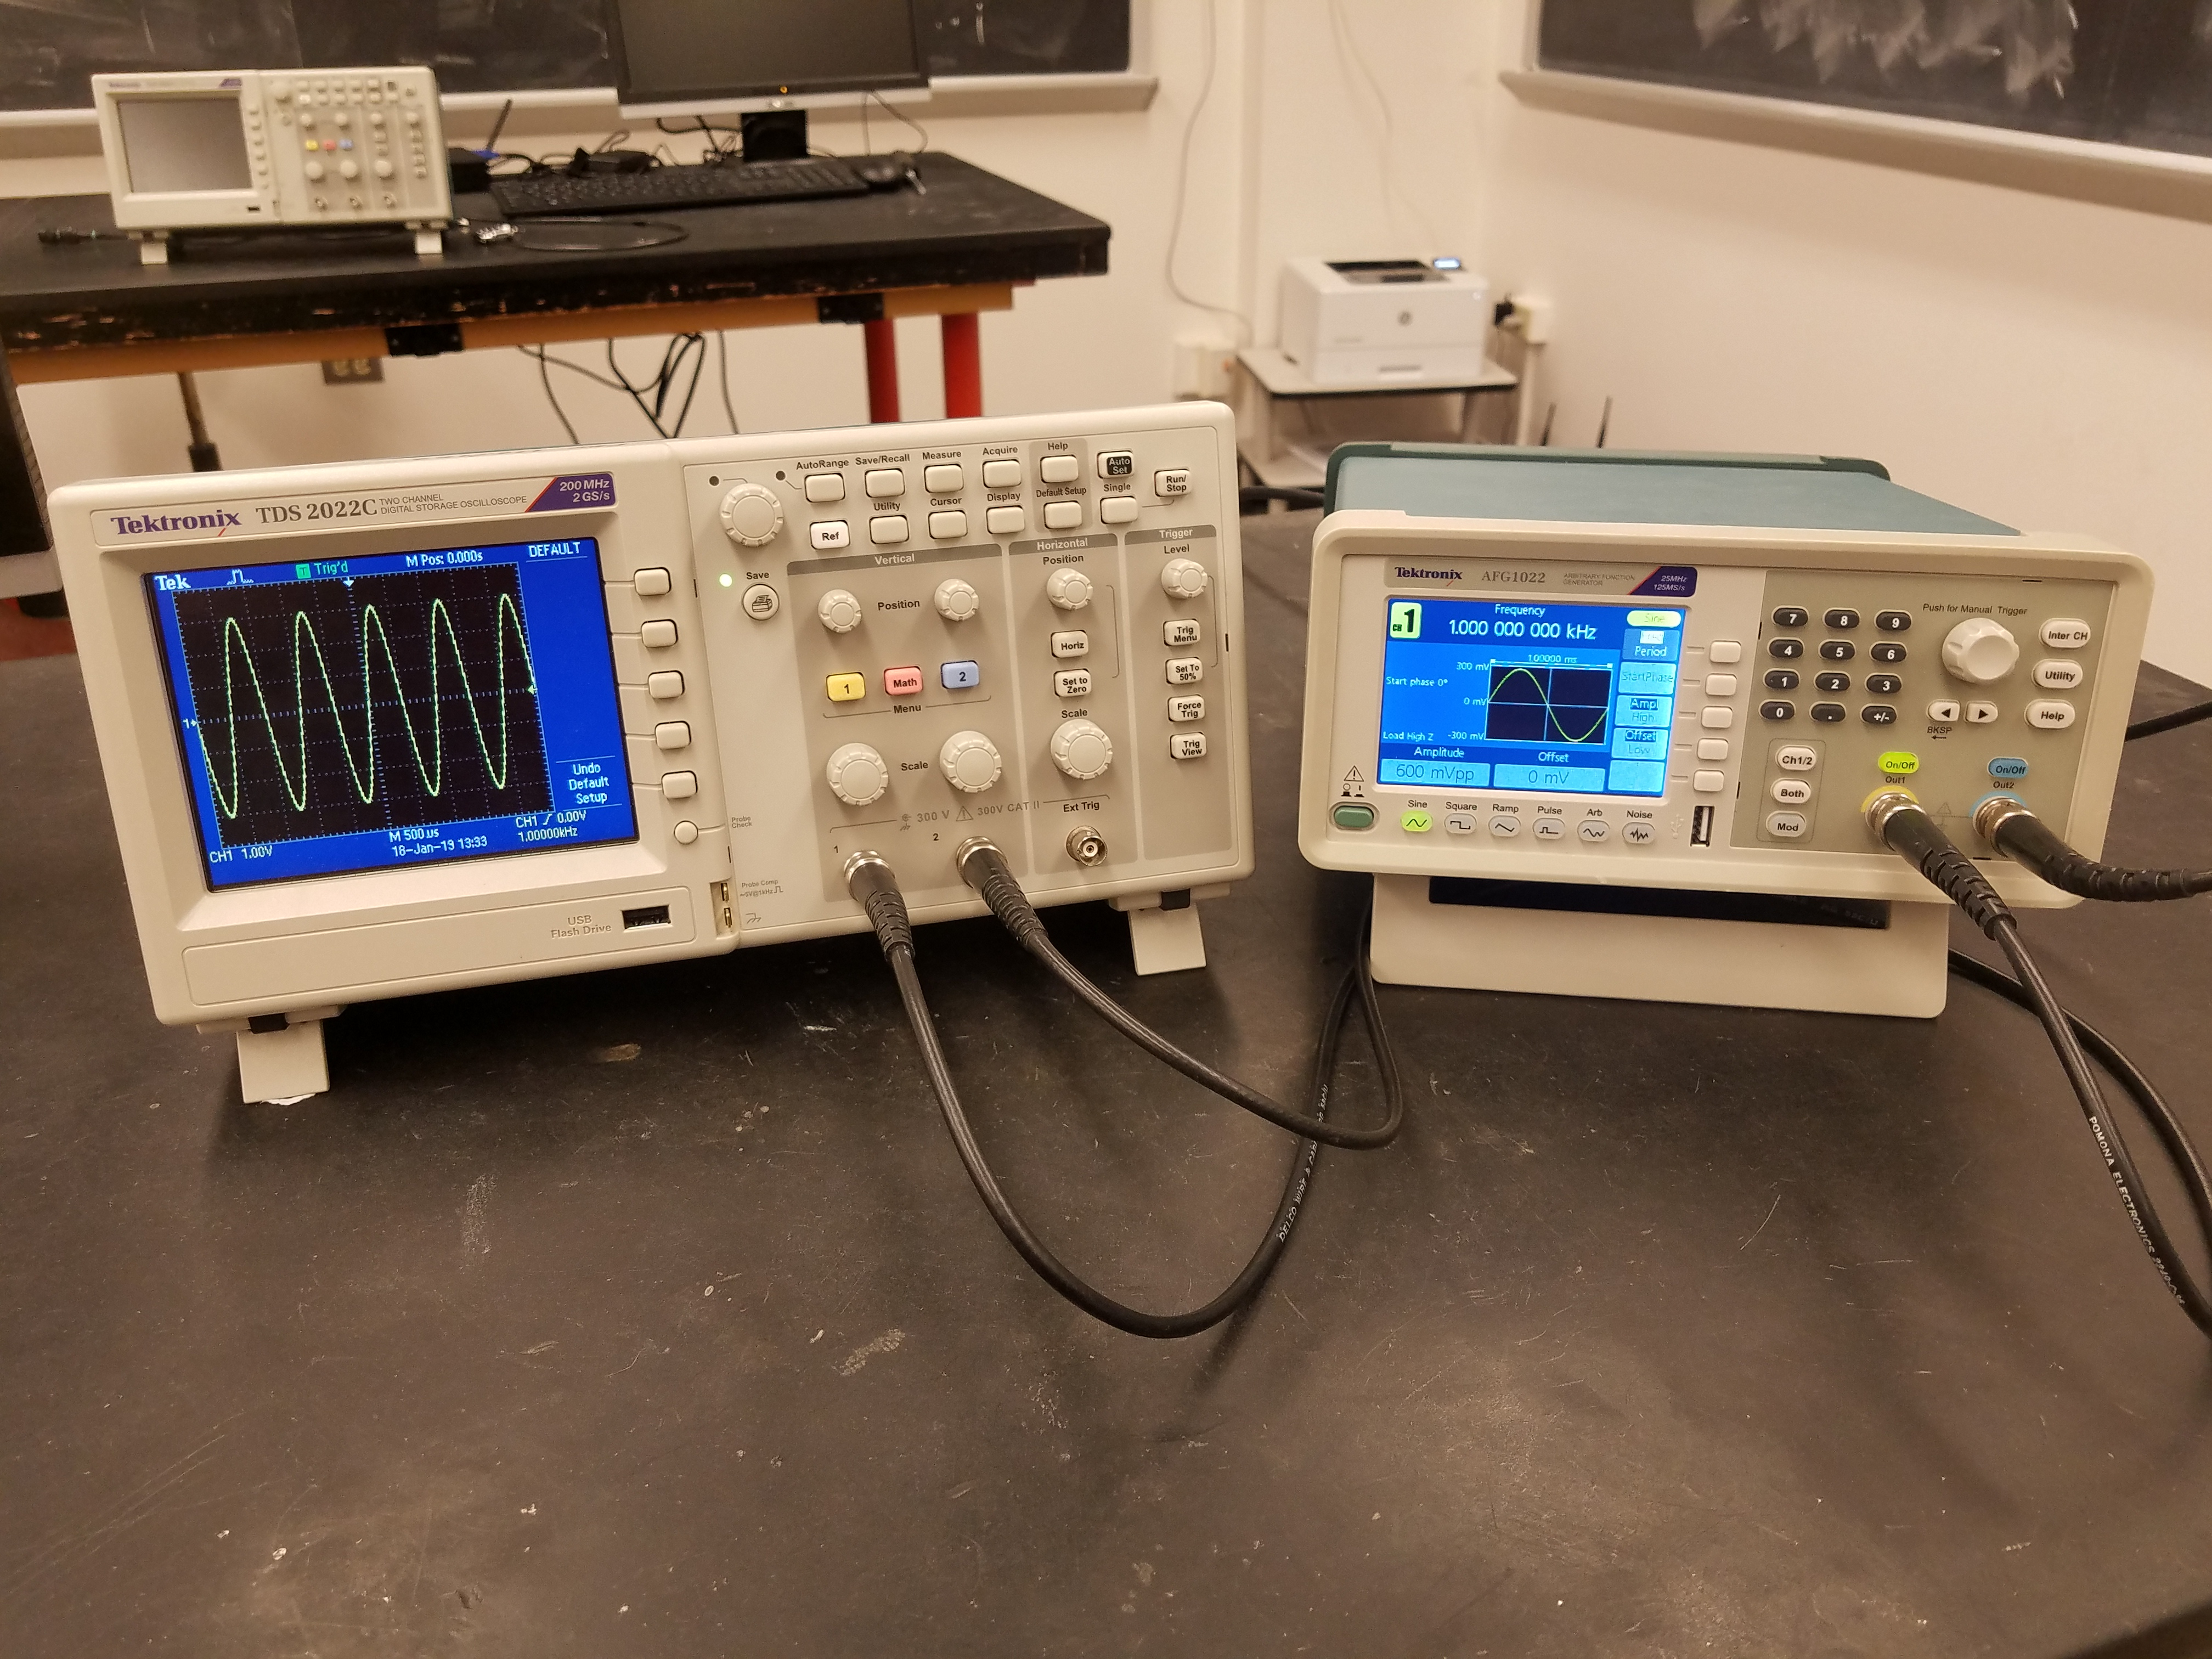
\includegraphics[width=0.45\textwidth]{figs/labs/lissajous/scope_setup.jpg} 
\caption{Connect the Channel 1 Output of your function generator directly to the Channel 1 input of your digital oscilloscope.}
\label{fig:scope_setup}
\end{center}
\end{figure}

Put your DMM aside.  Connect the Channel 1 output of your function
generator to the Channel 1 input of your digital oscilloscope.  Do the
same for Channel 2.  The setup is shown in Fig.~\ref{fig:scope_setup}.
Set your function generator to provide a $1~\rm kHz$ sine wave with
peak-to-peak voltage of $600~\rm mV$.  A DC offset of zero is implied
unless otherwise stated. Press the ``Default Setup'' button on your
digital scope.  You should immediately observe a sine wave on your
Digital scope just as in Fig.~\ref{fig:scope_setup}.

Press the button labeled ``Square'' on your function generator to
change the output from a Sine wave to a square wave and observe the
waveform on your scope.  Do the same for the Ramp and
Noise functions.  Then return to a Sine wave.

Press the yellow button labeled ``1'' several times.  This button
turns on and off the display of channel 1, and brings up the Channel 1
parameter menu.  Notice that the voltage scale for Channel 1 is
indicated as $1.0~V$.  This means that the difference between each
pair of consecutive horizontal lines corresponds to $1~V$.  We say
``One volt per division''.  By counting divisions, you should be able
to see that your waveform has a peak-to-peak voltage of $6~\rm V$.
Yet your function generator is set to produce $600~\rm mV = 0.6~\rm
V$.  Clearly someone is lying to us!

\begin{figure}[htbp]
\begin{center}
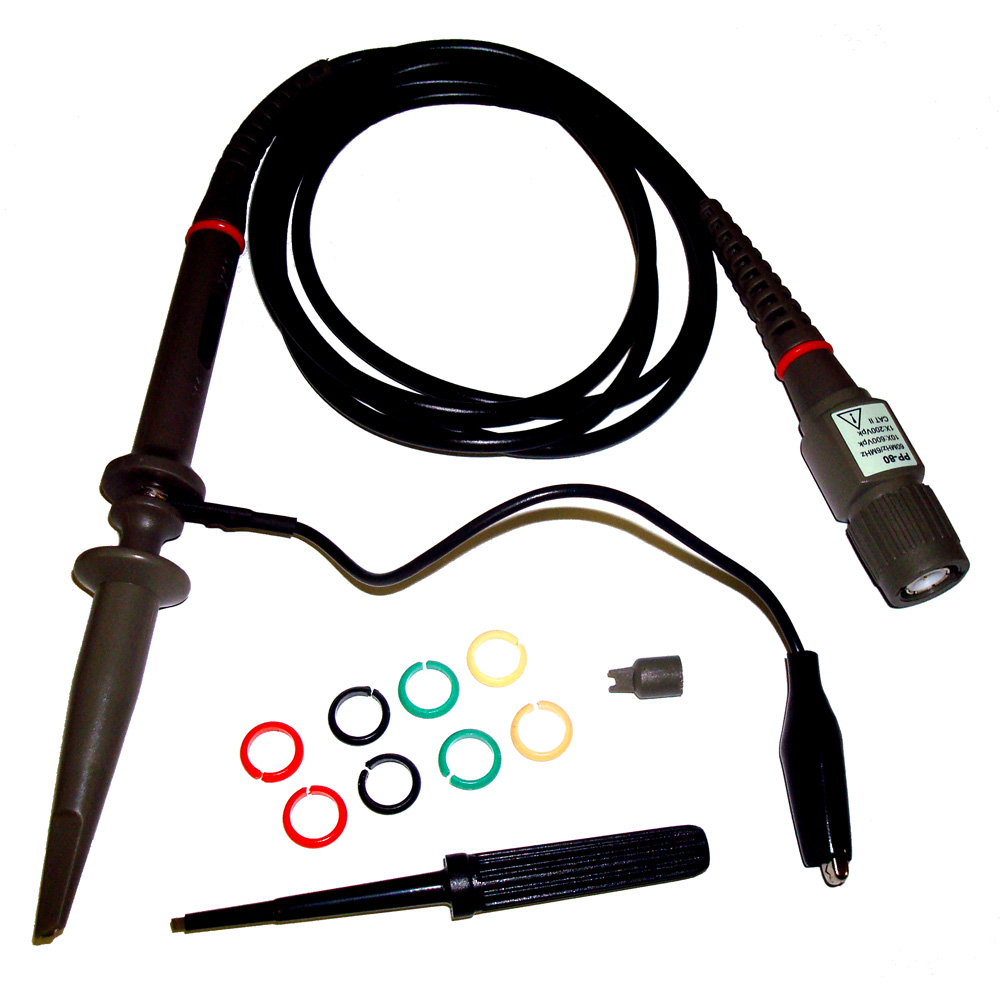
\includegraphics[width=0.45\textwidth]{figs/labs/lissajous/probe.jpg} 
\caption{An example scope probe.}
\label{fig:probe}
\end{center}
\end{figure}

Although we won't be using them in this lab, most sensitive
measurements with an oscilloscope are made using a scope probe, as
shown in Fig.~\ref{fig:probe}.  To protect the circuit being measured
from being effected by the insertion of the probe, there is usually a
large resistance in the probe.  This means that the oscilloscope
itself measures the output of a voltage divider, and the signal is
attenuated, most often by a factor of 10.  The oscilloscope simply
adjusts the voltage scale so that values you read are not attenuated.
To make consistent measurements, you simply have to make sure that the
oscilloscope is configured for the attenuation factor we are using.

In our case, we are connecting coaxial cables directly between the
oscilloscope and the function generator, and so there is no
attenuation.  But the default setup for the scope assumes that you are
using a probe with a $1/10$ attenuation, called a 10X probe.  Look at
the options next to the menu buttons and find the one that says
``Probe 10X Voltage''.  Press this menu button, and then press the
Attenuation button until it reads 1X, appropriate for a coaxial cable
with no attenuation factor.
\begin{figure}[htbp]
\begin{center}
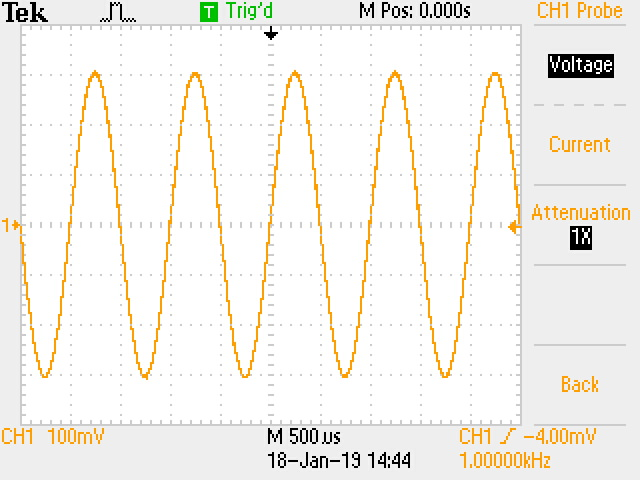
\includegraphics[width=0.45\textwidth]{figs/labs/lissajous/sine.jpg} 
\caption{Correctly scaled scope output.}
\label{fig:scopesine}
\end{center}
\end{figure}
The waveform is unchanged, but now the voltage scale is correctly set
to $100~\rm mV$.  And your signal now appears to be $600~\rm mV$,
consistent with the setting from your function generator, as shown in
Fig.~\ref{fig:scopesine}.  Next turn the knob labeled ``scale'' located
under the yellow channel ``1'' button.  Adjust this knob until the
scale for CH1 is listed as $200~\rm mV$ per division.  The apparent
size of the waveform will be reduced by a factor of two, because each
division is now $200~\rm mV$ and so your $600~\rm mV$ signal appears
three divisions high.

Next note that the function repeats every two divisions.  Since the
time scale is listed as $500~\rm \mu s$, the period is therefore $1~\rm
ms$, corresponding to a frequency of $1~\rm kHz$.  Adjust the time
scale, using the large knob in the Horizontal column, until the time
scale is $100~\rm \mu s$ per division.  This is still a $1~\rm kHz$
signal, but one period now takes up the entire display.

Using the multipurpose knob on your function generator, adjust the
frequency up to $10~\rm kHz$, and observe how the waveform changes.
Then adjust the voltage between about $100~\rm mV$ and $2~\rm V$
peak-to-peak.  When finished, leave the function generator producing a
$5~\rm kHz$ sine wave with $600~\rm mV$ peak-to-peak voltage.  Your
scope should remain at a voltage scale of $200~\rm mV$ and time scale
of $100~\rm \mu s$.  Next, set the DC offset of the signal on the function generator by pressing:
\begin{displaymath}
{\rm Offset \to 10 \to mV}
\end{displaymath}
Turn the multipurpose knob to adjust the DC offset between $-100~\rm
mV$ and $100~\rm mV$.  Your waveform will rise and fall on your scope
display.  By default, your scope includes the DC offset, but often this
is not what you want.  On your scope, press the button labeled
``Coupling DC'', until the DC becomes AC.  When AC coupled, the DC
component of your waveform is ignored.  AC coupling consists of using a capacitor to filter out the DC signal component from a signal with both AC and DC components. The capacitor must be in series with the signal. When AC coupled, observe that
changing the DC offset on the function generator does not change the
position of the waveform.

You can adjust the position of the waveform on your scope display using the small knobs
labeled ``Position'' to adjust the offset in vertical and horizontal.
Try this out.  To return a waveform to (0,0), notice that the offset is displayed while you are turning the knob.

\begin{plot} Save a scope trace with non zero vertical and horizontal offset. Insert your USB drive into the scope and press the Save button. 
\end{plot}

On your function generator, set the output to a $5~\rm V$ peak-to-peak
sine wave with frequency of $100~\rm kHz$.  Adjust the voltage scale
and time scale until you can clearly see the sine wave.

\section{Oscilloscope Trigger}

\begin{figure}[htbp]
\begin{center}
\begin{tabular}{cc}
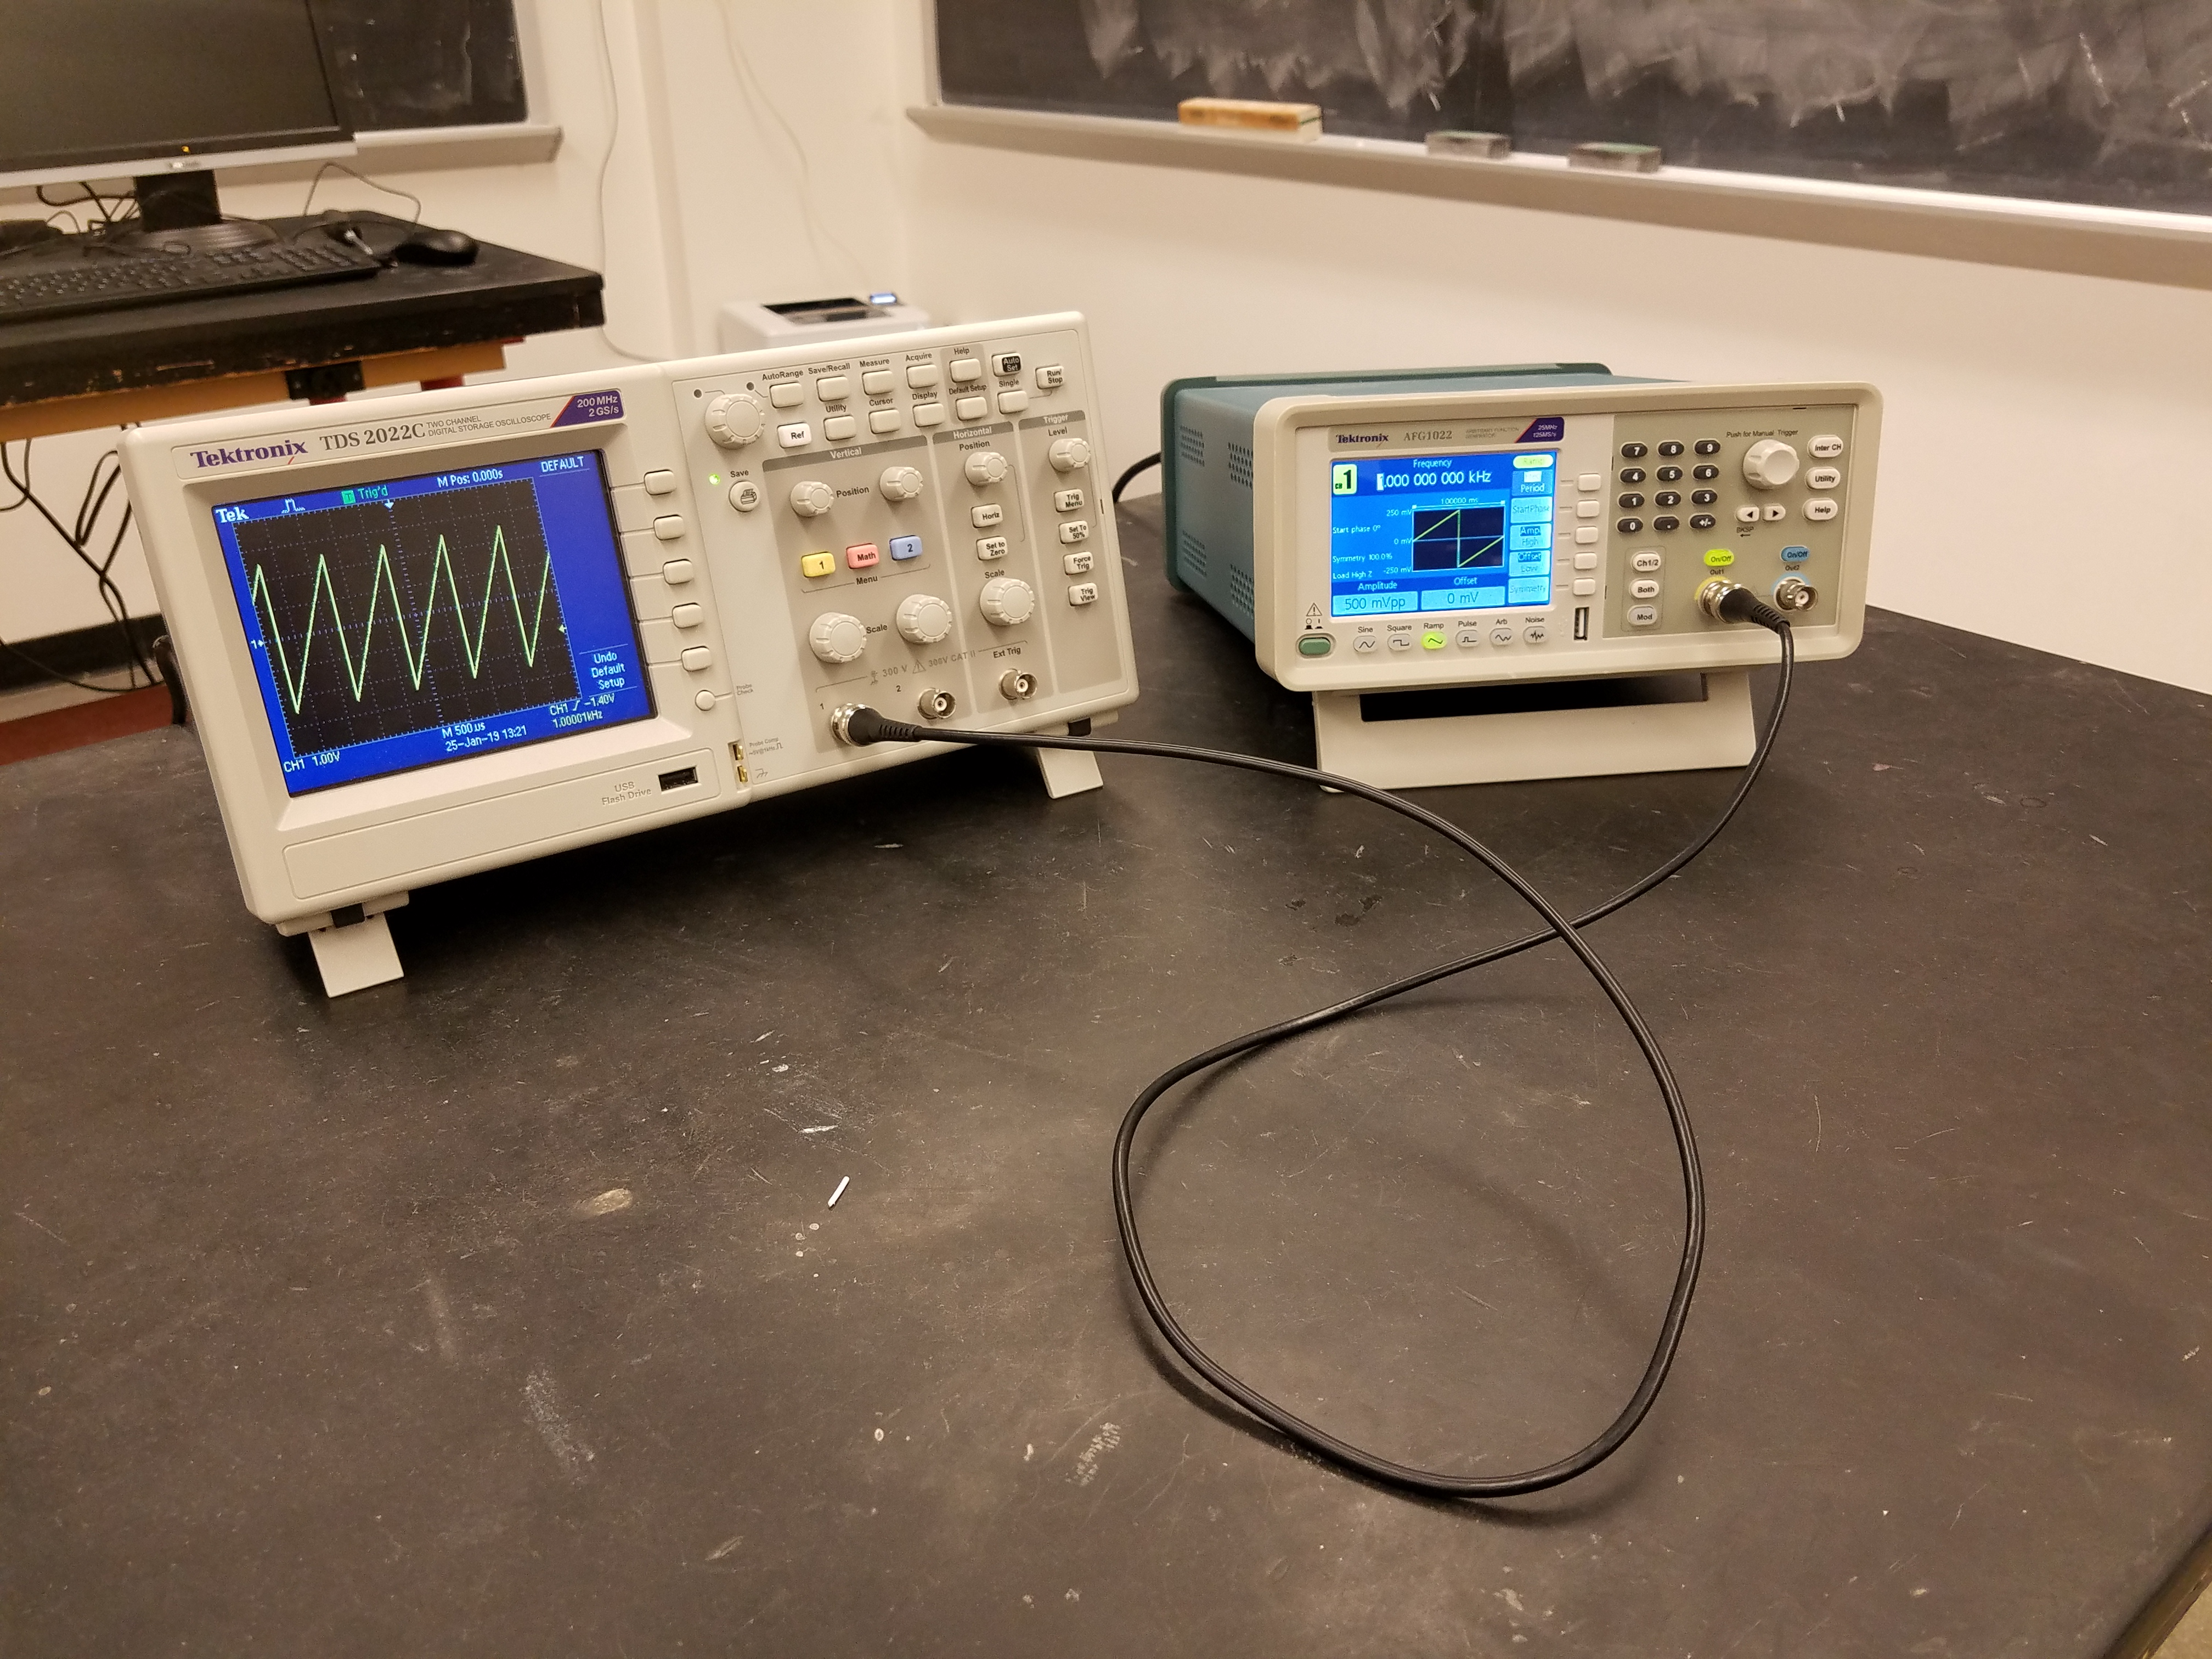
\includegraphics[width=0.40\textwidth]{figs/labs/transients/ramp_setup.jpg}  &
\begin{tikzpicture}
    \node[anchor=south west,inner sep=0] (image) at (0,0,0) {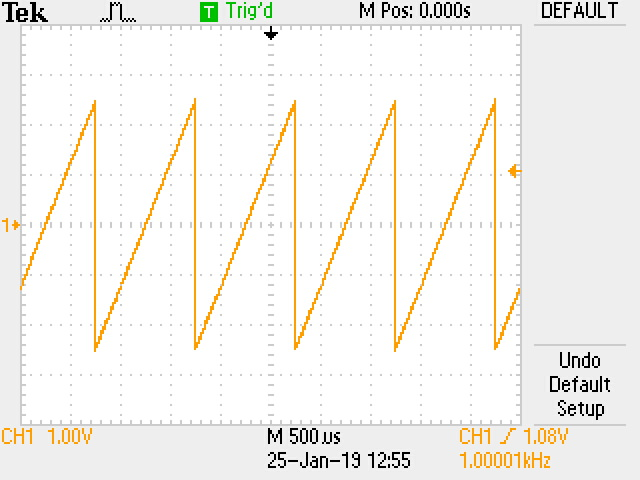
\includegraphics[height=0.25\textheight]{figs/labs/transients/trigger_ramp.jpg}};
    \node[left](X) at (0,5.3) {$t=0$};
    \draw (X.east) -- (3.3,5.7);
    \node[right](X) at (8.0,5.0) {\parbox{1cm}{Trigger \\ Threshold}};
    \draw (X.west) -- (6.5,3.9);
\end{tikzpicture}\\
(a) & (b) \\
\end{tabular}
\caption{(a) Setup for the scope trigger measurement, and (b) A scope trace triggered by the rising edge of ramp function.  The point $t=0$ is the location where the waveform first crosses the trigger thresholds, which is indicated by the arrow to the right.}
\label{fig:ramp_setup}
\end{center}
\end{figure}

Connect the output of Channel 1 on your function generator directly to
Channel 1 of your oscilloscope with a BNC cable, as in
Fig.~\ref{fig:ramp_setup}a.  Set your function generator to produce a
$1~\rm kHz$ Ramp function with a peak-to-peak amplitude of $600~\rm
mV$. While the Ramp function is selected, you will have an option
``Symmetry'' available.  Press the menu button next to Symmetry and
set the value to 100\%.  Turn on your oscilloscope and press the
``Default Setup'' button.  Recall that you need to
remember to (1) set your function generator to expect high-impedance
output, (2) enable the function generator output by pressing the
``On/Off'' button above the BNC connector for the channel, so that
button is lit (this is the last time these steps will be explicitly
mentioned.)  The ramp function should be immediately visible on your
scope.  Adjust the attenuation factor of Channel 1 to unity (X1)
appropriate for BNC cable and confirm the peak to peak amplitude and
the period are as expected (Leave Channel 2 alone for now.)

Your scope is continuously updating the display with the most recently
collected waveform, which at $1~\rm kHz$ is effectively instantaneous.
You may have wondered how these images all appear on the oscilloscope
with the exact same phase.  This crucial feature of your scope is a
result of its trigger feature, which we'll explore now.  Turn the knob
labeled ``Trigger Level'' and you should see the phase of your
waveform change. Notice that the trigger value and trigger type 
is displayed. Trigger value will be changing while you are turning the knob. 

As shown in Fig.~\ref{fig:ramp_setup}b, your scope display has an arrow at
the top of the display which indicates the point at which the trigger
condition was met for the current waveform, which is taken as $t=0$.
A second arrow, along the right side, indicates the trigger threshold.
Your scope is configured to trigger on the rising edge, which means it
will trigger at the instant where the trigger first goes above the
trigger threshold.

As you adjust the trigger threshold, the point at which the waveform
reaches this threshold changes.  Since $t=0$ is defined by the instant
at which the trigger condition is met, this effectively changes the
phase of your waveform.  As you adjust the threshold up and down, the
waveform moves forward and backward along the time axis.  This is an
example of an effect called ``time-slewing'', which is important to
consider when making time dependent measurements of wave forms, as we
will be doing today.

Notice what happens if you dial the threshold until it exceeds the
amplitude of your waveform.  Suddenly, your waveform will appear to
dance across the screen.  This is because your scope trigger is set to
``Auto'' trigger.  In this trigger mode, when too much time has passed
without the trigger condition being met, a waveform is displayed for
the current input using a random time for $t=0$.  This can be
convenient for finding a signal of unknown size and location.  Press
the ``Trigger Menu'' button, and then set the Trigger Mode to
``Normal'' by pressing the corresponding menu button.  In this Mode,
the waveform is not updated until a trigger is received.  While the
scope is in the Normal trigger mode, adjust the threshold so that it
is above the amplitude of the waveform.  You will notice that when the
trigger condition is not being met, the scope indicates the state
``Ready'' at the top of the screen, meaning that the scope is armed to
collect data when the trigger condition is met, but there has not
recently been a trigger.  Now move the threshold below the amplitude
for the waveform, and you should see the scope indicates the state
``Trig'd'', or triggered, on this display.  A common mistake for
students is to look at stale data, without realizing that the signal
is lost.  Avoiding this pitfall is one benefit of the Auto trigger
mode.

At times you may wish to start and stop the data acquisition.  This
can be accomplished using the ``Run/Stop'' button to pause and then
resume waveform acquisition.  Try this feature out now.  You can also
capture and display one single wave form by pressing the ``Single
Seq'' button.  This can be handy when looking at things like detector
pulses, which are different each time, and which may occur at a low
rate.  Resume normal data acquisition with the ``Run/Stop'' button.

Your scope trigger has the capability of triggering on either the
rising edge or the falling edge of the input.  When triggering on the
rising edge, the trigger fires at the instant the waveform first
exceeds the trigger threshold.  When triggering on the falling edge,
the trigger fires at the instant the waveform first falls below the
trigger threshold.  Using the appropriate menu button, set your scope
to trigger on the ``Falling'' edge.  You should observe that now the
$t=0$ occurs at the nearly straight vertical line in our ramp
function.  You'll also notice that adjusting the trigger threshold now
has no discernible effect on the phase of the waveform.  Triggering on
sharp edges eliminates the effect of time-slewing, a fact we will
exploit to make accurate time measurements.


\begin{plot} Save a scope trace when triggering on the falling edge.
\end{plot}

\noindent
This is a \textbf{sign-off point} for this lab. 

\section{Plotting}

Include your two scope traces in the python notebook. Make sure the date is clearly visible on each plot. Provide a full label for each plot which describes all the relevant information. 
You can display your scope traces in python using the Image library like this:
\begin{verbatim}
      from IPython.display import Image

       image = Image(filename='myscope.jpg') 
       display(image)
\end{verbatim}
This assumes that you copied your scope traces inside the jupyter notebook directory. 


\noindent
Please return all the components you took and cables to their place. Leave you workstation clean. 